% 4 章：SV モデルのための変分族
% 記述は実装と一致させている：src/sv_vi/advi.py（3 つの自前の族、conditional_factor）、banded.py（三重対角の O(T) 演算）、
% initialization.py（初期値）、guides.py（NumPyro 側の族）。
% 図 fig_sigma_roughness・表 tab_families は experiments/f4_family_illustration.py が生成。
\section{SV モデルのための変分族}\label{sec:family}

本章は本稿の中心であり、SV モデルの事後分布を近似する変分族を定義し、その性質を比較する。
\cref{sec:fam-requirements}で、第 2・3 章の議論から変分族に求められる要件を整理する。
\cref{sec:fam-meanfield,sec:fam-dense}で、汎用的な族（平均場、低ランク、フルランク）がなぜ SV モデルに向かないかを述べ、
\cref{sec:fam-structured}で、事後分布の三重対角構造を取り入れた構造化族と、その限界を説明する。
\cref{sec:fam-conditional}で、本稿が提案として扱う条件付き構造化族を定義し、
\cref{sec:fam-leverage,sec:fam-t}でそれを二つの拡張モデルに適用する。
\cref{sec:fam-summary}で各族を比較し、\cref{sec:fam-init}で初期値の設定を述べる。

本章では、第 3 章の ADVI に従い、大域パラメータを無制約空間の変数 $u \in \mathbb{R}^k$（$\theta = \theta(u)$）で表し、
推定する未知数を $z = (u, h_{1:T})$ とする（非中心化パラメータ化では $h$ の代わりに $x$）。
$k$ は大域パラメータの数で、基本 SV では 3、拡張モデルでは 4 である。

\subsection{変分族に求められる要件}\label{sec:fam-requirements}

第 2・3 章の議論から、SV モデルの変分族には次の四つが求められる。

\begin{enumerate}[label=(R\arabic*)]
  \item \textbf{$h_t$ の時間方向の相関を表せること}。
    $\theta$ を固定しても、隣り合う日の $h_t$ の事後相関は 0.9 程度に達する（\cref{tab:meanfield-gap}）。
    これを表せない族は、不確実性を過小評価するだけでなく、ELBO を通じてパラメータの推定そのものを偏らせる（\cref{sec:inf-vi}）。
  \item \textbf{$\theta$ と $h$ の事後的な依存を表せること}。
    とくに、$\sigma$ が $h$ の経路の滑らかさを決め、$\mu$ が $h$ の水準を決めるという依存（\cref{sec:model-structure}）である。
    これを表せないと、$\sigma$ の推定が偏り、その不確実性が過小評価される（\cref{sec:fam-structured}）。
  \item \textbf{計算量が $O(T)$ であること}。
    系列長 $T$ は数百〜数千であり、多数の銘柄を毎日推定することを考えると、1 ステップの計算量が $T$ の 2 乗以上で増える族は使いにくい。
    変分パラメータの数も $O(T)$ に抑えたい。数が多すぎると、雑音のある勾配での最適化が難しくなる。
  \item \textbf{パラメータ化の選び方に結果が左右されにくいこと}。
    中心化と非中心化のどちらを使うべきかを、銘柄やデータ期間ごとに判断しなくて済むことが、運用上は望ましい（\cref{sec:model-param}）。
\end{enumerate}

\cref{sec:model-structure}で見たように、(R1) と (R3) を同時に満たす鍵は、$h$ の事後分布の精度行列が三重対角であることにある。
(R2) を満たすには、$h$ の変分分布が $\theta$ に依存する形にしなければならない。
以下では、この観点から族を順に見ていく。

\subsection{平均場近似}\label{sec:fam-meanfield}

最も単純な族は、すべての変数を互いに独立な正規分布とする平均場近似である。
\[
  q(z) = \prod_{i=1}^{k} \Normal(u_i \mid m_i, s_i^2) \prod_{t=1}^{T} \Normal(h_t \mid m_{k+t}, s_{k+t}^2).
\]
変分パラメータは各変数の平均と標準偏差（正値を保つため対数で持つ）で、数は $2(k + T)$ である。
サンプリングは $z_i = m_i + s_i \epsilon_i$、エントロピーは $\sum_i \log s_i + \frac{k+T}{2}(1 + \log 2\pi)$ であり、計算量は $O(T)$ と最も軽い。
NumPyro の \code{AutoNormal} はこの族である。

しかし平均場近似は (R1) も (R2) も満たさない。
\cref{sec:inf-vi}で示したとおり、$h_t$ の時間方向の相関を表せないことから、ELBO は平均場近似が正確になる小さい $\phi$ を好み、
持続性の高いシナリオで $\phi$ を 0.05 程度にまで崩してしまう（真値 0.99）。
$\phi$ が崩れると、モデルは $h_t$ を日々ほぼ独立に動くものと解釈するので、$\sigma$ は 0.70 と真値（0.10）の 7 倍になり、
$h_t$ の事後標準偏差は NUTS の約 2 倍になる（\cref{sec:synthetic}）。
つまり平均場近似では、$h_t$ の不確実性はむしろ過大になり、「不確実性を過小評価する」という一般論とは逆の現れ方をする。
いずれにしても推定は使い物にならない。

\subsection{低ランク近似とフルランク近似}\label{sec:fam-dense}

平均場の対極にあるのが、すべての変数間の相関を許すフルランクの正規分布である。
\[
  q(z) = \Normal(z \mid m,\ L L^\top), \qquad L \text{ は対角が正の下三角行列}.
\]
次元を $d = k + T$ とすると、変分パラメータの数は $d + d(d+1)/2$ であり、$T = 1{,}000$ では約 50 万になる。
サンプリング $z = m + L\epsilon$ は $O(d^2)$、$\log q(z)$ の計算は三角行列の方程式を解くので $O(d^2)$ の計算量とメモリを要する。
族としては真の事後分布の正規近似を含むので、最適化が完全にできれば平均場よりはるかに良い近似が得られるはずである。
しかし実際には、50 万個のパラメータを、1 ステップ 4 サンプルの雑音のある勾配で最適化するのは難しい。
本稿の実験（NumPyro の \code{AutoMultivariateNormal}、20,000 ステップ）では、230 秒かけても $\phi = 0.24$ にとどまり、ELBO は比較したすべての族の中で最も低かった（\cref{sec:synthetic}）。

その中間として、共分散行列を「低ランク行列 + 対角行列」で表す低ランク近似がある。
\[
  q(z) = \Normal(z \mid m,\ W W^\top + D), \qquad W \in \mathbb{R}^{d \times r},\ D \text{ は対角}.
\]
本稿では NumPyro の \code{AutoLowRankMultivariateNormal} をランク $r = 10$ で使う。パラメータ数は $d(r+2)$、計算量は $O(d r)$（逆行列はウッドベリーの公式で計算）である。
低ランク近似は、少数の「共通因子」で多くの変数が一斉に動くような相関（例えば、全体の水準が上下する）を表すのは得意である。
しかし SV モデルの $h_t$ の相関は、隣り合う日どうしが強く、日が離れるにつれてなめらかに弱まる、という\textbf{局所的な}相関である。
AR(1) 過程の共分散行列の固有値は、周波数ごとのスペクトル密度 $\sigma^2/(1 - 2\phi\cos\omega + \phi^2)$ に対応してゆっくりと減衰するので、
少数の成分では局所的な相関を表しきれない。
実際、ランク 10 の低ランク近似は、平均場とほぼ同じ $\phi = 0.05$ に崩れた（\cref{sec:synthetic}）。

この二つの例は、\textbf{パラメータを増やすことと、事後分布の構造に合った族を選ぶことは別である}ことを示している。

\subsection{構造化近似：三重対角の精度行列}\label{sec:fam-structured}

\cref{sec:model-structure}で見たように、$\theta$ を固定したときの $h$ の事後分布は、三重対角の精度行列を持つ正規分布でよく近似できる。
そこで、$h$ の変分分布として、三重対角の精度行列を持つ正規分布を使う。
大域パラメータは次元が小さい（$k = 3$〜$4$）ので、フルランクの正規分布で表す。
\begin{equation}
  q(u, h) = \Normal(u \mid m_u,\ C C^\top)\; \Normal\!\left(h \mid m_h,\ (L L^\top)^{-1}\right).
  \label{eq:fam-structured}
\end{equation}
$C$ は $k \times k$ の下三角行列、$L$ は\textbf{下二重対角行列}（対角 $d_1, \dots, d_T > 0$ と、そのすぐ下の副対角 $s_1, \dots, s_{T-1}$ だけが 0 でない行列）である。
このとき精度行列 $L L^\top$ は三重対角になり、逆に三重対角の正定値行列は必ずこの形に分解できる（コレスキー分解）。
変分パラメータは $m_u$、$C$、$m_h$、$\log d_t$、$s_t$ で、数は $k + k(k+1)/2 + 3T - 1$ である。
この族は、精度行列のコレスキー因子に疎な構造を課した \textcite{tan2018} の変分近似の一例であり、\textcite{archer2015} の構造化近似とも同じ考え方に立つ。
本稿では、自前実装（\code{advi.py} の \code{structured}）と NumPyro のガイド（\code{guides.py}）の両方で実装し、同じ結果が得られることを確認した（\cref{sec:synthetic}）。

\paragraph{$O(T)$ の計算}
三重対角の精度行列を持つ正規分布は、密な行列を一切作らずに、すべての計算を $O(T)$ で行える（\code{banded.py}）。
\begin{itemize}
  \item \textbf{サンプリング}：$\epsilon \sim \Normal(0, I_T)$ について $L^\top x = \epsilon$ を解き、$h = m_h + x$ とする。
    $x$ の共分散は $L^{-\top} L^{-1} = (L L^\top)^{-1}$ なので、$h$ は確かに $\Normal(m_h, (LL^\top)^{-1})$ に従う。
    $L^\top$ は上二重対角なので、方程式は末尾から順に
    \[
      x_T = \epsilon_T / d_T, \qquad x_t = (\epsilon_t - s_t\, x_{t+1}) / d_t \quad (t = T-1, \dots, 1)
    \]
    と解ける（後退代入）。この漸化式は再パラメータ化の変換そのものであり、自動微分で $m_h$、$d_t$、$s_t$ についての勾配が得られる。
  \item \textbf{対数密度}：$\log \Normal(h \mid m_h, (LL^\top)^{-1}) = -\frac{T}{2}\log 2\pi + \sum_t \log d_t - \frac{1}{2} \lVert L^\top (h - m_h) \rVert^2$。
    $\log\det(LL^\top) = 2\sum_t \log d_t$ であり、$L^\top(h - m_h)$ の各成分は $d_t (h_t - m_{h,t}) + s_t (h_{t+1} - m_{h,t+1})$ と隣り合う 2 項だけで計算できる。
  \item \textbf{エントロピー}：$\mathcal{H} = \frac{T}{2}(1 + \log 2\pi) - \sum_t \log d_t$。対角成分の和だけで済む。
\end{itemize}

\paragraph{構造化近似の限界}
構造化近似は (R1) と (R3) を満たし、実際に $h_t$ の推定はかなり良い（\cref{sec:synthetic}）。
しかし $q(h)$ は $\theta$ に依存しないので、(R2) を満たさない。その影響は $\sigma$ に集中して現れる。

ELBO のうち $\theta$ に関係する部分は、$\E_{q(u)}\E_{q(h)}[\log p(h \mid \theta(u))] + \E_{q(u)}[\log p(\theta(u)) + \log\lvert J(u)\rvert] + \mathcal{H}[q(u)]$ である。
$q(h)$ が $\theta$ によらないので、$q(u)$ から見ると、第 1 項は「$q(h)$ から引いた $h$ の経路が\textbf{観測されている}ときの、AR(1) 過程のパラメータの対数尤度」を平均したものになる。
観測された $T-1$ 個の増分から $\sigma$ を推定するときの不確実性は、標準偏差でおよそ $\sigma / \sqrt{2(T-1)}$ である。
したがって $q(\sigma)$ の標準偏差もこの程度に縮む。
実際、一致度の実験（$T = 1{,}000$）での構造化近似の $\sigma$ の事後標準偏差は 0.0045 で、この式による値 $0.198/\sqrt{1998} = 0.0044$ とよく一致する。
実データの 1321（$T = 485$）でも、0.0077 に対して式は $0.239/\sqrt{968} = 0.0077$ を与える。
本来は $h$ そのものが不確実なので、$\sigma$ の事後標準偏差は NUTS では 0.027 と 6 倍も大きい。
構造化近似は、$h$ の不確実性が $\sigma$ の不確実性に波及する経路を断ち切っているのである。

$\sigma$ の値そのものも偏る。
上の見方では、$\sigma$ は「$q(h)$ から引いた経路の増分の大きさ」に合わせて決まる。
$q(h)$ は各日の $h_t$ の不確実性を覆うだけの広がりを持たなければならないが、その広がりを $\sigma$ に応じて変えることができないので、
$q(h)$ から引いた経路は真の事後分布からの経路より粗くなり、それに合わせて $\sigma$ が大きく推定される。
\cref{fig:sigma-roughness}は、一致度の実験と同じデータで、事後分布（変分分布）からのサンプルごとに $\sigma$ と $h$ の経路の粗さ $\sqrt{\mathrm{mean}_t (h_{t+1} - h_t)^2}$ を描いたものである。
NUTS では、$\sigma$ が大きいサンプルほど経路が粗く、両者の相関は 0.99 に達する。
これが (R2) で述べた $\sigma$ と $h$ の依存であり、$\phi \approx 1$ では増分 $h_{t+1} - h_t \approx \sigma \eta_t$ なので、粗さはほぼ $\sigma$ に等しい。
構造化近似では、この依存が完全に消え（相関 0.01）、点の雲は NUTS の分布から外れた $\sigma \approx 0.20$、粗さ $\approx 0.20$ の位置に小さく固まっている。

\begin{figure}[tbp]
  \centering
  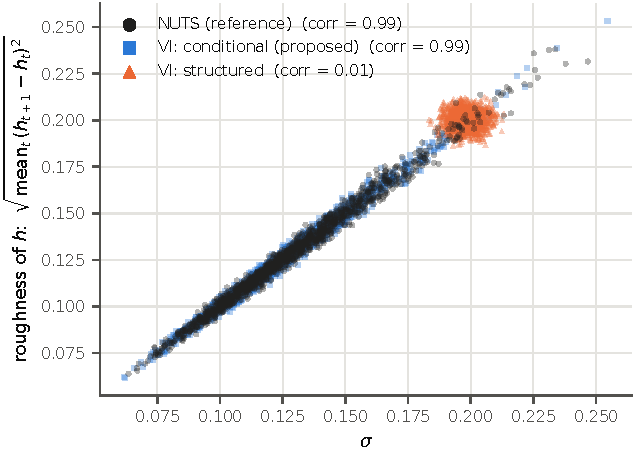
\includegraphics[width=0.75\linewidth]{figures/fig_sigma_roughness.pdf}
  \caption{$\sigma$ と $h$ の経路の粗さ $\sqrt{\mathrm{mean}_t (h_{t+1} - h_t)^2}$ の事後的な依存（一致度の実験の合成データ、高持続 $\phi = 0.99$、$\sigma = 0.10$、$T = 1{,}000$）。
    各点は事後分布（変分分布）からの 1 サンプル（各 1,500 点を表示）。括弧内は全サンプル（NUTS 16,000、VI 各 4,000）での相関係数。
    NUTS は 4 連鎖、ウォームアップ 2,000 の後に 32,000 回更新して 8 回に 1 回を保存。VI は 20,000 ステップ。}
  \label{fig:sigma-roughness}
\end{figure}

\subsection{条件付き構造化近似（提案）}\label{sec:fam-conditional}

構造化近似の問題は、$q(h)$ が $\theta$ に依存しないことにあった。
そこで、$h$ の変分分布を $\theta$ に条件付けた形にする。本稿では次の族を考え、\textbf{条件付き構造化変分族}と呼ぶ。
\begin{equation}
  q(u, h) = \Normal(u \mid m_u,\ C C^\top)\; q\!\left(h \mid \theta(u)\right), \qquad
  q(h \mid \theta) \;\propto\; p(h \mid \theta) \prod_{t=1}^{T} \Normal\!\left(\tilde y_t \;\middle|\; h_t,\ \lambda_t^{-1}\right).
  \label{eq:fam-conditional}
\end{equation}
$p(h \mid \theta)$ は SV モデルの AR(1) 事前分布そのもの、$\tilde y_t \in \mathbb{R}$ と $\lambda_t > 0$ は変分パラメータである。
$q(h \mid \theta)$ は、「AR(1) の事前分布を持つ $h$ について、$\tilde y_t$ という値を精度 $\lambda_t$ で観測したときの事後分布」という形をしている。
$\tilde y_t$ を\textbf{擬似観測}、$\lambda_t$ をその\textbf{精度}と呼ぶ。
真の観測 $y_t$ は $h_t$ について非線形・非正規な情報を与えるが（\cref{sec:model-likelihood}）、それを各日ごとの正規分布の形の情報で置き換えたもの、と見ることができる。
変分パラメータは $m_u$、$C$、$\tilde y_{1:T}$、$\log\lambda_{1:T}$ で、数は $k + k(k+1)/2 + 2T$ であり、構造化近似（$3T$ 程度）より少ない。

\paragraph{$q(h \mid \theta)$ の具体形}
\cref{eq:fam-conditional}の右辺の対数をとると、
\[
  \log q(h \mid \theta) = -\frac{1}{2}(h - \mu\mathbf{1})^\top Q_{\mathrm{AR}}(\phi, \sigma)\,(h - \mu\mathbf{1}) - \frac{1}{2}\sum_{t=1}^{T} \lambda_t (h_t - \tilde y_t)^2 + \text{定数}
\]
であり（$Q_{\mathrm{AR}}$ は\cref{eq:ar1-precision}の三重対角行列、$\mathbf{1}$ はすべて 1 のベクトル）、$h$ の二次式である。
したがって $q(h \mid \theta)$ は正規分布で、平方完成により
\begin{equation}
  \begin{gathered}
  q(h \mid \theta) = \Normal\!\left(h \;\middle|\; m(\theta),\ P(\theta)^{-1}\right), \\
  P(\theta) = Q_{\mathrm{AR}}(\phi, \sigma) + \diag(\lambda), \qquad
  m(\theta) = P(\theta)^{-1}\left( Q_{\mathrm{AR}}(\phi, \sigma)\, \mu\mathbf{1} + \lambda \odot \tilde y \right)
  \end{gathered}
  \label{eq:fam-conditional-gauss}
\end{equation}
を得る（$\odot$ は成分ごとの積）。
精度行列 $P(\theta)$ は三重対角行列に対角行列を足したものなので、やはり三重対角であり、構造化近似と同じく $O(T)$ で扱える。
平均は $m(\theta) = \mu\mathbf{1} + P(\theta)^{-1}\{\lambda \odot (\tilde y - \mu\mathbf{1})\}$ とも書ける。
擬似観測の情報（$\lambda$）が AR(1) の事前分布の精度に比べて小さい日には、$h_t$ の平均は長期水準 $\mu$ に引き寄せられ、大きい日には $\tilde y_t$ に近づく。

\paragraph{$\theta$ との依存}
この族では、$h$ の分布が $\theta$ の関数として自動的に変わる。
\begin{itemize}
  \item $\sigma$ が小さいと、$Q_{\mathrm{AR}}$ の成分（$\propto 1/\sigma^2$）が大きくなり、隣り合う $h_t$ を強く結びつける。
    すなわち $h$ の経路は\textbf{滑らかに}なり、平均も擬似観測の細かな変動を追わなくなる。$\sigma$ が大きければその逆である。
  \item $\mu$ が大きくなると、平均 $m(\theta)$ は事前分布の寄与の分だけ上に動く。
  \item $\phi$ が 1 に近づくと、遠く離れた日どうしの結びつきも強くなる。
\end{itemize}
これがまさに (R2) の依存である。
\cref{fig:sigma-roughness}のとおり、条件付き構造化近似は、$\sigma$ と経路の粗さの相関（0.99）と、両者の同時分布の形を NUTS とほぼ同じに再現している。

\paragraph{ラプラス近似との関係}
この族の形は、\cref{sec:model-structure}のラプラス近似から自然に導かれる。
$\theta$ を固定し、$h$ の事後分布の最頻値 $\hat h$ をニュートン法で求めることを考える。
各日の観測の対数尤度を現在の点 $\hat h_t$ のまわりで二次近似すると、
\[
  \log p(y_t \mid h_t) \approx \text{定数} + g_t (h_t - \hat h_t) - \frac{c_t}{2} (h_t - \hat h_t)^2
  = \text{定数} - \frac{c_t}{2}\left(h_t - \Bigl(\hat h_t + \frac{g_t}{c_t}\Bigr)\right)^2,
\]
\[
  g_t = -\frac{1}{2} + \frac{y_t^2}{2} e^{-\hat h_t}, \qquad c_t = \frac{y_t^2}{2} e^{-\hat h_t}
\]
となる（$g_t$、$c_t$ は 1 階・2 階微分の符号を変えたもの）。
これは「値 $\hat h_t + g_t / c_t$ を精度 $c_t$ で観測した」ときの対数尤度と同じ形であり、ニュートン法の各ステップは、AR(1) の事前分布とこの擬似観測による正規分布の事後分布を計算することに等しい。
ニュートン法が収束した点では、ラプラス近似の正規分布\cref{eq:laplace-precision}は、\cref{eq:fam-conditional-gauss}で $\tilde y_t = \hat h_t + g_t/c_t$、$\lambda_t = c_t$ としたものに一致する。
つまり条件付き構造化族は、\textbf{各 $\theta$ でのラプラス近似と同じ形の分布を、すべての $\theta$ について同時に表す族}である。
ただし擬似観測とその精度は $\theta$ によらない共通の値であり、それを（ラプラス近似のように最頻値から決めるのではなく）ELBO の最大化で決める。
擬似観測が $\theta$ によらないことはこの族の近似の一つであり、例えば $\theta$ によって擬似観測の最適な値が大きく変わる場合には誤差が生じる。

\paragraph{サンプリングとエントロピーの計算手順}
ELBO の推定値は、1 サンプルあたり次の手順で計算する（\code{advi.py} の \code{conditional\_factor} と \code{draw}）。
すべての手順が $O(T)$ であり、自動微分によって変分パラメータ全体についての勾配が得られる。
\begin{enumerate}[label=(\arabic*)]
  \item $\epsilon_u \sim \Normal(0, I_k)$ から $u = m_u + C\epsilon_u$ を作り、$\theta = \theta(u)$ に変換する。
  \item 三重対角行列 $P(\theta) = Q_{\mathrm{AR}}(\phi, \sigma) + \diag(\lambda)$ の対角 $a_t$ と副対角 $b_t$ を作る。
  \item コレスキー分解 $P(\theta) = L L^\top$ を漸化式
    $d_1 = \sqrt{a_1}$、$s_t = b_t / d_t$、$d_{t+1} = \sqrt{a_{t+1} - s_t^2}$
    で計算する（$L$ は下二重対角で、対角 $d_t$、副対角 $s_t$）。
  \item 平均 $m(\theta)$ を、$P(\theta) m = Q_{\mathrm{AR}}\mu\mathbf{1} + \lambda \odot \tilde y$ を前進代入（$L w = $ 右辺）と後退代入（$L^\top m = w$）で解いて求める。
  \item $\epsilon_h \sim \Normal(0, I_T)$ について $L^\top x = \epsilon_h$ を後退代入で解き、$h = m(\theta) + x$ とする。
  \item 対数同時密度\cref{eq:advi-jacobian}を $(u, h)$ で評価する。
\end{enumerate}
エントロピーは、同時分布のエントロピーの連鎖律
\[
  \mathcal{H}[q(u, h)] = \mathcal{H}[q(u)] + \E_{q(u)}\!\left[\mathcal{H}[q(h \mid \theta(u))]\right], \qquad
  \mathcal{H}[q(h \mid \theta)] = \frac{T}{2}(1 + \log 2\pi) - \sum_{t=1}^{T} \log d_t(\theta)
\]
で計算する。第 1 項は $q(u)$ が正規分布なので解析的に書け、第 2 項の期待値は (1) で引いた $M$ 個の $u$ での標本平均で推定する（不偏推定）。
第 2 項の中の $d_t(\theta)$ は (3) で計算済みなので、追加の計算はほとんどない。
こうして $M = 4$ 個のサンプルで ELBO を推定し、その勾配で Adam の 1 ステップを進める。
1 ステップの計算は、$M$ 本の長さ $T$ の漸化式（\code{jax.lax.scan}）を数回回すことに相当する。

\paragraph{パラメータ化に依存しないこと}
非中心化パラメータ化（$x = (h - \mu)/\sigma$）で同じ族を使う場合は、上の手順で $h$ を作ったあと $x = (h - \mu)/\sigma$ と変換する。
$\theta$ を固定すれば、これは $h$ のアフィン変換なので、$x$ の分布も三重対角の精度行列を持つ正規分布であり、エントロピーは $T\log\sigma$ だけ減る（実装ではこの補正を入れている）。
このとき $(\theta, h)$ の同時分布としては、中心化で作った $q$ とまったく同じ分布族になる。
ELBO は未知数の可逆な変数変換によって変わらない（$\log p$ と $\log q$ が同じヤコビアンの分だけ変わり、打ち消し合う）ので、
\textbf{条件付き構造化族では、中心化・非中心化のどちらを使っても同じ最適解と同じ ELBO が得られる}。
これに対して、平均場・構造化・フルランクの族では、$h$ に正規分布を当てるか $x$ に当てるかで $(\theta, h)$ の同時分布の族そのものが変わる（$h = \mu + \sigma x$ は $\theta$ と $x$ について非線形なので）。
例えば非中心化の構造化族では、$h$ の広がりが $\sigma$ に比例して変わるので (R2) の依存の一部が表せるようになり、$\sigma$ の不確実性の過小評価が緩和される（\cref{app:settings}）。
条件付き構造化族は、そうした依存を最初から族に組み込んでいるので、パラメータ化を選ぶ必要がない（R4）。
この性質は数値的にも確認しており、中心化と非中心化で推定結果は一致する（\cref{app:settings}）。

\paragraph{位置付け}
条件付き構造化族は、\cref{sec:intro-related}で述べた既存の考え方の組み合わせである。
局所変数（ここでは $h$）の変分分布を大域パラメータに条件付けるという構造は \textcite{tan2020} と同じであり、
「事前分布 × 正規分布の擬似観測」という表現は、\textcite{johnson2016} が状態空間モデルの構造化 VI でニューラルネットワークに出力させた共役な因子を、自由な変分パラメータで置き換えたものにあたる。
また \textcite{loaizamaya2022} は、潜在変数について近似ではなく正確な条件付き事後分布 $p(h \mid y, \theta)$ を使う族を提案しているが、
SV モデルでは $p(h \mid y, \theta)$ からの正確なサンプリング自体に MCMC などが必要になる。
本稿の族は、その代わりに $\theta$ ごとのラプラス近似と同じ形の正規分布を使うことで、すべての計算を閉じた形・$O(T)$ に保っている。
手法としての新しさよりも、SV モデルの構造（AR(1) 事前分布の三重対角の精度行列と、$\sigma$ が滑らかさを決めるという依存）を変分族に正しく入れることの効果を示すことが、本稿の主眼である。

\subsection{レバレッジ SV への拡張}\label{sec:fam-leverage}

レバレッジ SV では、$\theta$ を固定したときの $h$ の事後分布の形が変わる。
\cref{eq:sv-leverage-state}を使うと、同時分布は
\[
  p(y, h \mid \theta) = p(h_1 \mid \theta) \prod_{t=1}^{T-1} p(h_{t+1} \mid h_t, y_t, \theta) \prod_{t=1}^{T} p(y_t \mid h_t)
\]
と分解できる（$y_t$ の周辺分布 $p(y_t \mid h_t)$ は $\Normal(0, e^{h_t})$ のまま）。
$h$ の事後分布の「事前分布にあたる部分」は、もはや $p(h \mid \theta)$ ではなく、
イノベーションの分散が $\sigma^2(1 - \rho^2)$ に縮み、平均に $\rho\sigma\, y_t e^{-h_t/2}$ というリターンに連動したドリフトが加わった遷移 $p(h_{t+1} \mid h_t, y_t, \theta)$ の積になる。

基本 SV の族をそのまま使い、$q(h \mid \theta)$ を $\rho$ によらない AR(1) 事前分布から作ると、$\rho$ と $h$ の依存がまったく表せない。
本稿の予備実験では、この最初の版は $\rho$ の推定値をほぼ 0（$-0.08$。真値 $-0.5$）に潰してしまった。
第 3 章で見た平均場の $\phi$ と同じ理屈で、ELBO が「$q$ の近似が正確になる $\rho = 0$」を好んだためと考えられる。

そこで、$q(h \mid \theta)$ の遷移部分をレバレッジ SV の遷移に合わせて
\begin{equation}
  \begin{aligned}
  q(h \mid \theta) \;\propto\;& \Normal\!\left(h_1 \;\middle|\; \mu, \frac{\sigma^2}{1-\phi^2}\right)
    \prod_{t=1}^{T-1} \Normal\!\left(h_{t+1} \;\middle|\; \mu + \phi(h_t - \mu) + \rho\sigma\,\tilde e_t,\ \sigma^2(1 - \rho^2)\right) \\
    &\times \prod_{t=1}^{T} \Normal\!\left(\tilde y_t \;\middle|\; h_t, \lambda_t^{-1}\right)
  \end{aligned}
  \label{eq:fam-leverage}
\end{equation}
とする。真のドリフトの中の標準化リターン $y_t e^{-h_t/2}$ を、新たな変分パラメータ $\tilde e_t$（$t = 1, \dots, T-1$）で置き換えたものである。
こうすると $q(h \mid \theta)$ は再び正規分布になり、精度行列はイノベーションの標準偏差を $\sigma\sqrt{1 - \rho^2}$ とした AR(1) の精度行列に $\diag(\lambda)$ を足した三重対角行列、
平均の計算ではドリフト $\rho\sigma\tilde e_t$ が右辺の 1 次の項に加わるだけで、計算はすべて $O(T)$ のまま変わらない。
$\rho$ が変わると、$h$ の遷移の不確実性（$\sigma^2(1 - \rho^2)$）とドリフトの大きさ（$\rho\sigma\tilde e_t$）が連動して変わるので、$\rho$ と $h$ の依存の主要な部分が表せる。
この修正により、予備実験の $\rho$ の推定値は $-0.37$ まで改善した。

それでも、合成データの復元実験では、$\rho$ は真値より 0 の側に約 25\% 縮んで推定される（$T = 2{,}000$ で偏り $+0.13$、95\% 区間の被覆率 0.35、事後標準偏差は NUTS の 0.65 倍。\cref{sec:synthetic}）。
残る偏りの原因は、真のドリフト $\rho\sigma\, y_t e^{-h_t/2}$ が $e^{-h_t/2}$ を通じて $h_t$ に\textbf{非線形に}依存することにある。
$h_t$ が高い日ほど同じリターンでも標準化リターンは小さく、ドリフトも小さくなるが、$\tilde e_t$ を $h_t$ によらない定数とした正規分布の族ではこの依存が表せない。
ステップ数や学習率を変えても偏りは変わらなかったので、最適化の問題ではなく族の表現力の限界である。
これを解消するには、遷移が $h_t$ に非線形に依存する変分族（例えば正規化フロー）が必要になり、今後の課題とする（\cref{sec:conclusion}）。
なお実データでは、$\rho$ の推定値の差は NUTS との比較で 0.02〜0.06 程度であった（\cref{sec:empirical}）。

実装上の注意として、$\tilde e_t$ の初期値を 0 にしてはならない。
ドリフトは $\rho\sigma\tilde e_t$ という積の形をしているので、$\rho$ についての勾配は $\tilde e_t$ に比例し、$\tilde e_t$ についての勾配は $\rho$ に比例する。
$\rho$ の初期値は 0 なので、$\tilde e_t$ も 0 から始めると両方の勾配が 0 になり、最適化がそこから動かない（鞍点）。
本稿では、$\tilde e_t$ の初期値を、$h$ の初期値 $h^{(0)}_t$ による標準化リターン $y_t e^{-h^{(0)}_t/2}$ とした。

\subsection{\texorpdfstring{$t$}{t} 誤差の SV への適用}\label{sec:fam-t}

$t$ 誤差の SV モデルでは、状態方程式は基本 SV と同じであり、観測の尤度だけが変わる。
条件付き構造化族の $q(h \mid \theta)$ は、事前分布の部分（$p(h \mid \theta)$）と擬似観測の部分からなり、観測の尤度の形は擬似観測が吸収するので、族の形を変える必要はない。
自由度 $\nu$ は大域パラメータとして $u$ に加え（$\nu = 2 + e^{u_\nu}$）、$q(u)$ を 4 次元のフルランクの正規分布にするだけである。
$t$ 分布の対数尤度は $h_t$ についての曲率に上限がある（\cref{sec:model-likelihood}）ので、極端なリターンの日には最適な擬似観測の精度 $\lambda_t$ が小さくなり、その日の観測の影響が自動的に弱まると期待される。

\subsection{変分族の比較}\label{sec:fam-summary}

\cref{tab:families}に、本稿で比較する変分族の性質をまとめる。
パラメータ数は、基本 SV（$k = 3$）、$T = 1{,}000$ のときに実際に最適化される変分パラメータの数である（下三角行列は $k(k+1)/2$ 個と数える）。
条件付き構造化族は、本稿で比較する族の中で (R1)〜(R4) のすべてを満たす唯一の族であり、しかもパラメータ数は平均場とほとんど変わらない。
その違いを生んでいるのは、パラメータの数ではなく、モデルの構造（AR(1) の事前分布）を変分族の中にそのまま組み込んでいることである。

\begin{table}[tbp]
  \centering
  \caption{変分族の比較（基本 SV、$T = 1{,}000$）。
    (R1)〜(R4) は\cref{sec:fam-requirements}の要件で、○は満たす、△は一部のみ、×は満たさない。
    (R1) は $h_t$ の時間方向の相関、(R2) は $\theta$ と $h$ の依存（フルランクは正規分布で表せる線形の依存のみ、低ランクは少数の因子を通じた依存のみ）、
    (R3) の計算量は 1 サンプルあたりのサンプリングと密度計算の計算量、パラメータ数は実際に最適化される変分パラメータの数（下三角行列は $k(k+1)/2$ 個と数える）、
    (R4) の不変性は中心化と非中心化で $(\theta, h)$ の分布の族が変わらないこと。}
  \label{tab:families}
  \footnotesize
  \setlength{\tabcolsep}{4pt}
  \begin{tabular}{lllcccrc}
\toprule
 & \multicolumn{2}{c}{共分散（精度）の構造} & (R1) & (R2) & \multicolumn{2}{c}{(R3)} & (R4) \\
\cmidrule(lr){2-3} \cmidrule(lr){6-7}
変分族 & $q(\theta)$ & $q(h)$ & 時間相関 & $\theta$--$h$ 依存 & 計算量 & パラメータ数 & 不変性 \\
\midrule
平均場 & 対角 & 対角 & × & × & $O(T)$ & 2,006 & × \\
低ランク（$r=10$） & \multicolumn{2}{c}{$WW^\top + D$} & △ & △ & $O(Tr)$ & 12,036 & × \\
フルランク & \multicolumn{2}{c}{密な共分散 $LL^\top$} & ○ & △ & $O(T^2)$ & 504,509 & × \\
構造化 & フルランク & 三重対角の精度 & ○ & × & $O(T)$ & 3,008 & × \\
条件付き構造化 & フルランク & $Q_{\mathrm{AR}}(\theta) + \diag(\lambda)$ & ○ & ○ & $O(T)$ & 2,009 & ○ \\
\bottomrule
\end{tabular}

\end{table}

\subsection{初期値}\label{sec:fam-init}

VI は最適化なので、初期値が結果や収束の速さに影響しうる。
本稿では、すべての手法（NUTS を含む）で共通の初期値を使う（\code{initialization.py}）。
\begin{itemize}
  \item \textbf{$h$ の初期値}：$\log y_t^2 = h_t + \log\varepsilon_t^2$ と $\E[\log\varepsilon_t^2] \approx -1.27$（\cref{sec:model-likelihood}）から、
    $h^{(0)}_t$ を $\log(y_t^2 + c) + 1.27$ の 10 日移動平均とする。$c = 0.1 \times \overline{y^2}$ は、リターンが 0 の日に対数が発散するのを防ぐための小さな定数である。
  \item \textbf{$\theta$ の初期値}：$\phi = 0.95$、$\sigma = 0.2$、$\mu = h^{(0)}$ の平均、レバレッジ SV では $\rho = 0$、$t$ 誤差の SV では $\nu = 10$。
    NUTS では、これを無制約空間で連鎖ごとに標準偏差 0.1 だけずらして使う（\cref{sec:inf-mcmc}）。
\end{itemize}
変分パラメータの初期値は、族ごとに次のように決める（\code{advi.py} の \code{init\_params}）。
\begin{itemize}
  \item \textbf{$q(u)$}（構造化・条件付き構造化）：平均は $\theta$ の初期値を無制約空間に写したもの、$C = 0.1\, I$。
  \item \textbf{平均場}：$h$ の平均は $h^{(0)}$、標準偏差は $1/\sqrt{\Lambda_{tt}}$（$\Lambda = Q_{\mathrm{AR}}(\theta^{(0)}) + \frac{1}{2}I$）。これは正規分布の目標に対する平均場の最適解（\cref{sec:inf-vi}）である。大域パラメータの標準偏差は 0.1。
  \item \textbf{構造化}：$m_h = h^{(0)}$、$L$ は $Q_{\mathrm{AR}}(\theta^{(0)}) + \frac{1}{2}I$ のコレスキー因子。
  \item \textbf{条件付き構造化}：$\tilde y_t = h^{(0)}_t$、$\lambda_t = 1/2$、レバレッジ SV では $\tilde e_t = y_t e^{-h^{(0)}_t/2}$。
\end{itemize}
ここで 1/2 は、観測 1 つが $h_t$ について持つ期待フィッシャー情報 $\E[y_t^2 e^{-h_t}]/2 = 1/2$ である（\cref{sec:inf-vi}）。
つまり、精度の初期値は「$\theta^{(0)}$ でのラプラス近似」を大まかに真似たものになっている。
初期値への感度は\cref{app:settings}で確認している。

時点ごとの変分パラメータ（$\tilde y_t$、$\lambda_t$、$\tilde e_t$ など）は、推定期間を 1 日ずらしたときに 1 つずらして次の日の初期値に使える。
これを使った日次の再推定（warm start）は\cref{sec:system}で扱う。
